\documentclass[a4paper]{article}
\usepackage{lipsum}
\usepackage{url}
\usepackage{graphicx}
\usepackage{listings}
\usepackage{indentfirst}
\usepackage{enumerate}
\usepackage{multicol}
\lstset{language=Haskell}
\usepackage[margin=2cm]{geometry}
\graphicspath{ {images/} }
\renewcommand{\familydefault}{\sfdefault}

\title{COMP4075/G54RFP Coursework Part II}
\date{5\textsuperscript{th} December 2018}
\author{Benjamin Charlton --- psybc3 --- 4262648}

\usepackage{fancyhdr}

\pagestyle{fancy}
\fancyhf{}
\lhead{Benjamin Charlton | psybc3 | 4262648}
\rhead{G54RFP}
\cfoot{\thepage}

\begin{document}

\maketitle

\section{Task II.1 --- Dining Philosophers}

\subsection{Solution Design}
The problem is to develop a system simulating a number of philosophers at a table all alternating between thinking and eating.
The issue is the limited amount of eating implements (sporks were used in this solution as to distinguish from forking threads) and the fact each philosopher needs 2 sporks to eat.
\par
The main idea behind the solution is the use of Software Transactional Memory (STM), where each spork is held in a piece of STM\@.
If a philosopher is hungry they will wait until they can grab both sporks at the same time and then begin eating.
After they have finished eating they return the sporks to the table (adding them back into the relevant STM) so others can get them if required.
\par
The solution is designed to generate a number of sporks equal to the number of philosophers.
This means that the system can work with an arbitrary number of philosophers that is \( \ge 1\) as 1 philosopher will cause a deadlock as they want 2 sporks but only 1 exists.

\subsection{Sample Output}
Here is some sample output for my solution running with 7 philosophers around the table.
It shows the first 50 lines of output and the time of each line being printed.
\begin{center}
    \begin{multicols}{2}
        \lstinputlisting[firstline=0, lastline=50]{Suppliments/dpOutput.txt}
    \end{multicols}
\end{center}

\subsection{Implementation}

\subsubsection{Helper Functions}
\paragraph{Microseconds to Seconds}
This function converts a integer representing a number of seconds to the same time in microseconds
\lstinputlisting[language=Haskell, firstline=3, lastline=4]{reportIICode.hs}
\paragraph{Getting a String containing the current time}
This function uses the library Data.Time to get the current time and format it.
\lstinputlisting[language=Haskell, firstline=6, lastline=9]{reportIICode.hs}
\paragraph{Printing a Philosopher doing an Action}
This function prints a formatted string with the current time, the philosophers name and their intent (Thinking, Hungry, Eating)
\lstinputlisting[language=Haskell, firstline=11, lastline=15]{reportIICode.hs}
\paragraph{Delaying a Philosopher and Printing}
This function will print how long the philosopher thread will be delayed (used to simulate the thinking/eating time) and then delays the thread for the given number of seconds.
\lstinputlisting[language=Haskell, firstline=17, lastline=23]{reportIICode.hs}

\subsubsection{Philosopher function}
The main outline of the philosopher function is an infinite loop by recursively calling itself without changing any of the inputs.
It takes a string for the philosophers name and the pair of sporks that the philosopher will use while doing some IO action.
The work that happens during this function is described in the following paragraphs but this code segment gives an idea of the overall structure.
\lstinputlisting[language=Haskell, firstline=26, lastline=30]{reportIICode.hs}
\paragraph{Thinking}
The thing the philosopher does first is thinking.
This is done by simply declaring the intent and then delaying for a random number of seconds (between 1 and 10).
\lstinputlisting[language=Haskell, firstline=32, lastline=34]{reportIICode.hs}
\paragraph{Hungry}
Once the philosopher has stopped thinking they will become hungry.
While hungry they try and take the 2 sporks on either side of them, this action is done atomically to ensure that their are no dead locks.
\lstinputlisting[language=Haskell, firstline=36, lastline=40]{reportIICode.hs}
\paragraph{Eating}
Once the philosopher has both sporks they can start eating, this happens in the same way as the thinking with a stating the intent and then delaying for a random amount of time.
Once they have finished eating, they return the sporks by atomically putting them back correctly.
Although the value replaced strictly doesn't matter they return the same value to the TMVar.
\lstinputlisting[language=Haskell, firstline=42, lastline=47]{reportIICode.hs}

\subsubsection{Main}
The main function is what is executed when the program first runs, this is split into 3 major sections.
\paragraph{Generating pairs of sporks}
In the first 2 lines of the main function all of the synchronising variables are created.
First of all the correct number of sporks equal to the number of philosophers and numbers them, the numbering isn't required for the system to run but allows for an easy and efficient way of creating enough TMVars in a map.
After this the sporks are zipped into relevant pairs so that they can be passed onto the philosophers.
\paragraph{Forking philosophers}
The next lines deals with the forking separate threads for each of the philosophers.
It zips the philosopher and pairs of sporks together running each one under the philosopher function.
For each element in this list it will fork a separate thread to run the philosopher under.
\paragraph{Blocking Main}
The final is a way to allow main to continue running as if main ever terminates the philosopher threads will also end.
By continuously calling threadDelay it means that main will never terminate.
\lstinputlisting[language=Haskell, firstline=50, lastline=56]{reportIICode.hs}

\subsection{STM vs Classical Solutions}

\subsubsection{Why STM is free of deadlocks}
During attempts to pick up sporks both actions are done atomically, meaning that there is no way for a philosopher to have access to a single spork.
If a philosopher can't access the sporks it will simply wait and retry until it can access them both.

\subsubsection{Resource Hierarchy Solution}
A pro of using STM a hierarchy solution is that a STM doesn't generate a situation where many philosophers are holding a single spork waiting for the other to become available.
This is because an STM allows for both sporks to be picked up at the same time allowing more of the philosophers eating at the same time.
As stated in the wikipedia article if there was 5 philosophers at a table all hungry at the same it would mean that only 1 philosopher would have access to both sporks required for eating, in the STM system 2 philosophers would manage to get access to both required sporks.
This situation doesn't get any better for more philosophers as in the hierarchy system there will always only be 1 philosopher able to get both resources, this would often result in a long wait time for the others to eat and the available fork trickling one by one around the table, only having one philosopher eating at a time.
The STM system would allow \( \frac{1}{2}\) of the philosophers to eat at once giving a higher utilisation of resources and sooner freeing of those resources for other philosophers.
\par
Another problem with the hierarchy system is if at a later date a thread requires more resources it needs to systematically free the higher resources are require them all starting at the lowest resource.
This can result in complex code to write as you have to remember to acquire resources in the correct order.
With an STM this can be resolved by freeing all of the resources and then reacquiring them all atomically, as the order doesn't matter its much simpler to reacquire the resources you need correctly.

\subsubsection{Arbitrator Solution}
The arbitrator solution creates a single synchronisation variable that tells the philosophers if they are allowed to pick up sporks.
This simplifies the amount of synchronisation needed to be managed but can reduce the parallelism as several philosophers that could safely pick up sporks have to wait and it also makes the synchronising logic more complex.
\par
You can leave the synchronisation logic fairly simple if you simply let a single philosopher attempt to pick up their sporks at once and if they fail to do so let them continue trying until they succeed (This works as replacing sporks is always allowed).
The problem with this solution is the reduction in parallelism achieved as many threads are simply waiting for their turn, an issue that is reduced with the STM solution.
\par
You could create a more sophisticated synchronisation logic if you allowed philosophers to revoke its permission to collect sporks if it fails to collect them.
This would allow the arbitrator to give another philosopher a chance to try and access their sporks and they may succeed.
This would increase parallelism but not to the same levels as the STM solution, while also requiring much more complex logic leaving more places where bugs could occur.

\section{Task II.2 --- Electronic Calculator}

\subsection{Design}
The Electronic Calculator use the threepenny framework to display the relevant data as a webpage, allowing the user to interact with the program with a better user experience.
The framework uses functional reactive programming to avoid the call back soup.
This allows the UI to be generated and interacted with in a functional manner by the underlying system.
\par
The core calculator part is written using many functional techniques to get it to work properly.
There are data type for both the calculation (A tree of operations) and the calculator (current calculation and the previous answer).
This allows for new features to be easily added by inserting them into the current calculation system.

\subsection{ScreenShots}
\paragraph{ScreenShot 1}
This screenshot shows the calculator in its initial state.
The default answer and calculation are both 0.
The buttons are layed out in some order allowing a user to easily distinguish between the digits, operations, recall functions, constants and evaluating.
\begin{center}
    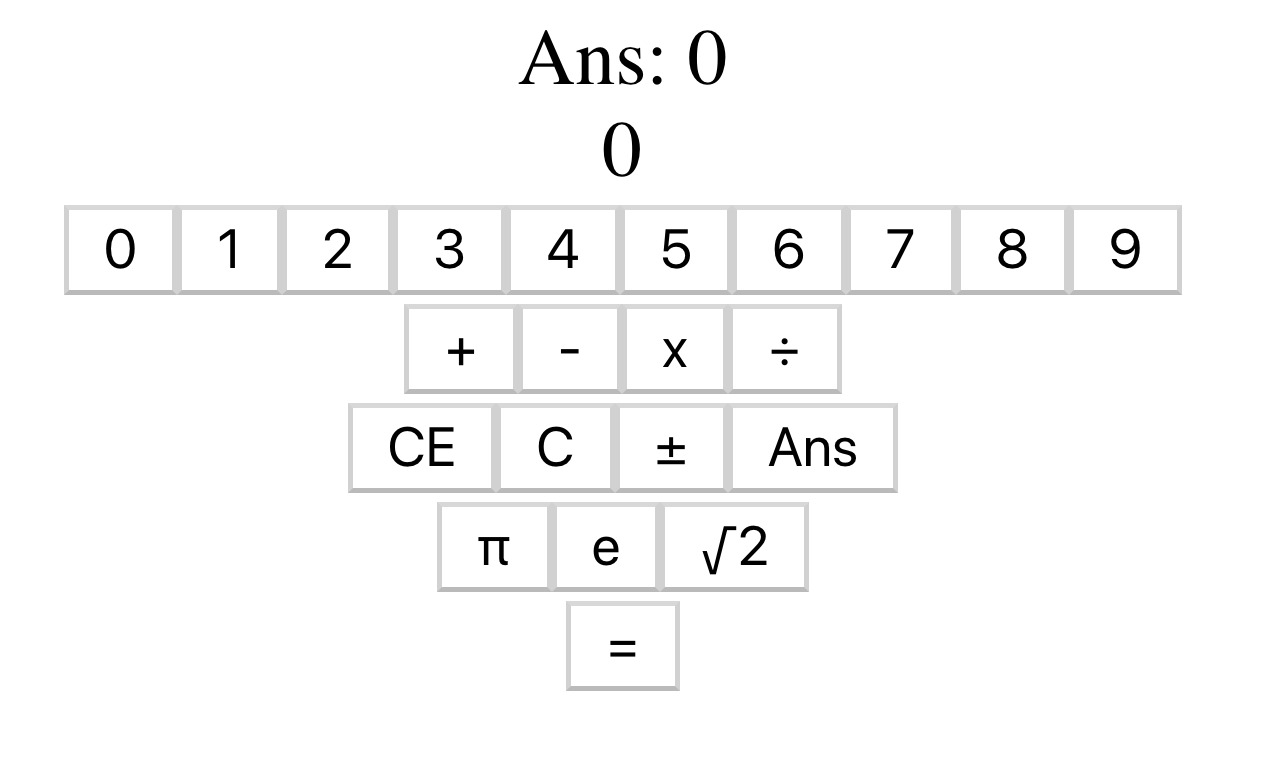
\includegraphics[width=10cm]{Suppliments/calculator1.png}
\end{center}
\paragraph{ScreenShot 2}
This screenshot shows how the calculation is built up during input but before the equals button is pressed.
The system uses the correct mathematical symbols to allow for the used to easily read the calculation.
\begin{center}
    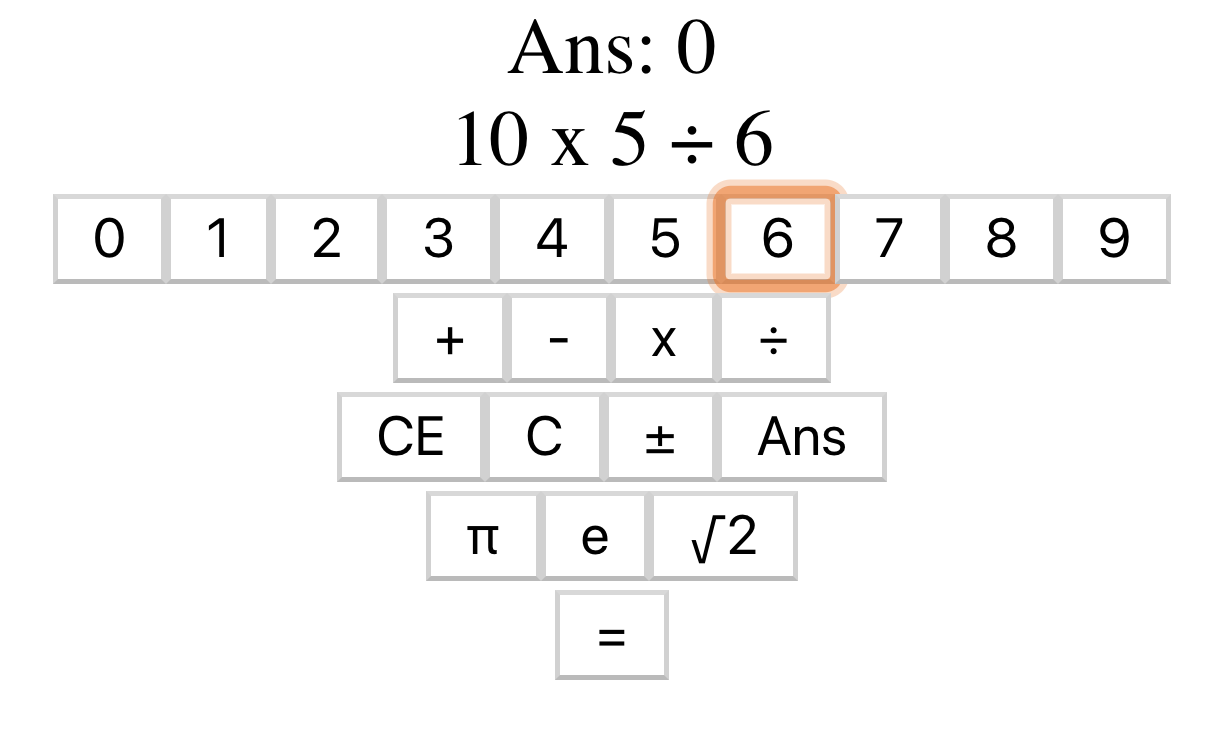
\includegraphics[width=10cm]{Suppliments/calculator2.png}
\end{center}
\paragraph{ScreenShot 3}
This screenshot shows how the results are shown in the answer field as a single number, as well as the usage of some of the constants in a calculations.
Although in this example the answer is a decimal number, if the result doesn't need to be show as a decimal it will round the double and present the integer.
\begin{center}
    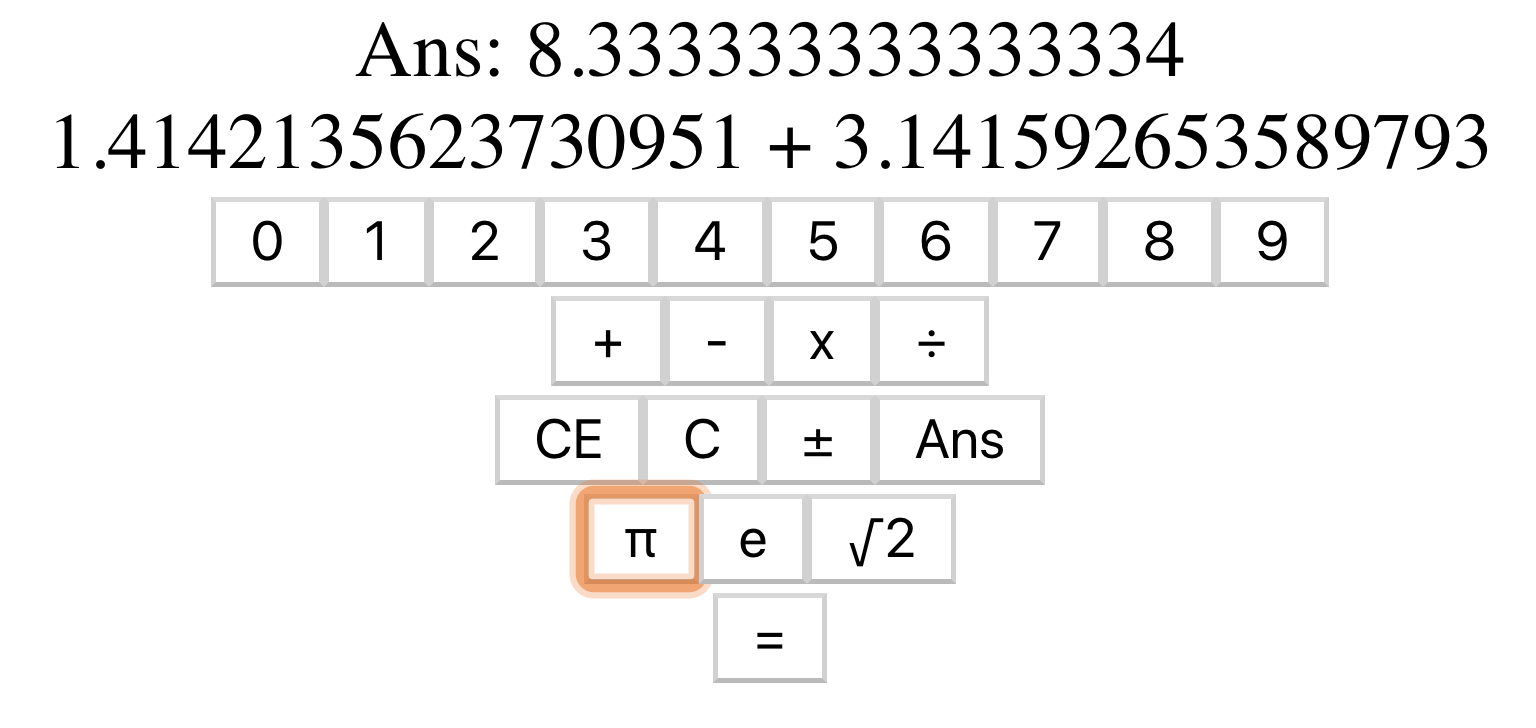
\includegraphics[width=10cm]{Suppliments/calculator3.png}
\end{center}

\subsection{Implementation}
\subsubsection{Basic Functions}
\paragraph{Handling large Numbers}
The calculation uses doubles to store the any number within it, allowing to handle large numbers that are at least 10 digits long.
The issue with this is that as the numbers get to extreme values (both as big numbers or small numbers) the doubles lose precision
It is unlikely that users will be using numbers this extreme so it is left as is.
\par
When a digit button is pressed it will change the last number in the calculation to have the digit appended to it.
The first function is a helper function allowing the digit to be added to the calculator type.
The addDigitCalc function recursively looks through the tree finding the last number (right most in the display) and updates it.
As the number is a double it updates it by shifting the number 1 point up (*10) and then adding the new digit to the end.
\lstinputlisting[language=Haskell, firstline=59, lastline=66]{reportIICode.hs}

\paragraph{Basic Operations}
The basic operators are stored in the calculation as a tree structure, where the node is the operator and the children are the right and left side of it respectively.
The leaf nodes are all numbers so ultimately you have an operator as a node and 2 numbers as the children to apply the operator too.

\paragraph{Sign Changing}
The sign changing operation is stored in the same calculation tree as the other operators.
The sign change is the node and it has a single child which is the calculation to change the sign of.
\par
As 2 sign changes would cancel each other out the function to add the changing sign to the calculation tree will pattern match on the current calculation to see if it already has its sign changed.
If it does it will remove the sign change, otherwise it will add it to the front of the calculation.
\lstinputlisting[language=Haskell, firstline=102, lastline=104]{reportIICode.hs}

\paragraph{Reset and Clear Last Entry}
These buttons function very similarly to each other.
clearEntry takes the current calculator and simply returns it with the same current calculation with a reset the previous answer to 0.
The clear calculator function returns a calculator with its default setting of a clear calculation and 0 as the previous answer.
\lstinputlisting[language=Haskell, firstline=69, lastline=73]{reportIICode.hs}

\paragraph{Evaluation}
The main evaluation function takes in the current calculator and returns an evaluated calculator with the new answer and the calculation set to the default.
This is aided by a helper evaluation function that takes in a calculation and returns the answer as a double.
The evaluator recursively works down the tree by evaluating the children nodes and then combining them with the relevant operator.
Leaf nodes with numbers are the base case simply returning the number they contain.
Any part of the calculation that needs its sign changed is simply multiplied by -1 to get the correct result.
Finally all of the binary operators are applied, the definition for add is given but the other operators work similarly by evaluating each side of the calculation and combining them with the operator.
\lstinputlisting[language=Haskell, firstline=76, lastline=83]{reportIICode.hs}

\subsubsection{Advanced Functions}
\begin{itemize}
    \item Decimal
    \item Memory
    \item Precedence
\end{itemize}
\paragraph{Decimal Fractions}
To handle decimal numbers, all numbers are evaluated as doubles.
This is a simple and easy way to leverage the strong type system of Haskell to give a sensible answer.
As all of the numeric operations are covered in the prelude for Haskell there where no complications in evaluating doubles as opposed to another numeric type such as ints.

\paragraph{Memory}
Memory in this calculator is only handled for accessing the previous answer.
This is done by changing the right most number in the calculation to whatever is held in the answer field.
This is done by calling a function that takes the current calculator and returns the modified calculator.
A helper function is used to help manipulate the calculation by pattern matching on the tree and recursively following the right most path till it finds the correct number to change.
\lstinputlisting[language=Haskell, firstline=86, lastline=93]{reportIICode.hs}

\paragraph{Precedence}
Standard precedence is not implemented in the current version of this calculator, opting instead to evaluate it from left to right.
This does result in some incorrect calculations as compared to standard mathematics but the calculator is self consistent.
\par
With the way the evaluation function works and how the calculation is stored it wouldn't be impossible to create a new evaluate function that handles precedence.
This could be achieved by restructuring the tree and evaluating it according to standard precedence.
This is due to the types being handled would still be the same and the evaluate function not having any side effects.
We can be confident that simply changing this function to one that performs standard precedence wouldn't change the rest of the system.

\subsubsection{Extra Features}
\paragraph{Constants}
Some key mathematical constants were added as they are a common feature of calculators.
To add these were simple working in the same way that adding the answer as the current number works.
\lstinputlisting[language=Haskell, firstline=96, lastline=99]{reportIICode.hs}

\subsection{Code Explanation}
\subsubsection{Main}
Main simply uses the Threepenny library to start the GUI and bind the web-server to correct address and port so it can handle new connections.
It then runs the setup function that will add elements to the GUI and event handlers.

\subsubsection{Additional helper functions for setup}
\paragraph{Button Creation}
As creating a button was a common task this function would take in the string and then create the button UI Element.
\lstinputlisting[language=Haskell, firstline=108, lastline=109]{reportIICode.hs}

\paragraph{Showing the Calculator}
To show the calculator in the UI it was best to present it as a string.
Separate functions were made to display the answer and the calculation parts so that they could be given to separate labels.
\par
By leveraging the type classes of Haskell the calculation could be made an instance of show be converted to a string that way.
\par
To make the UI look nicer all numbers a checked to see if they are whole numbers.
If they are then we round the double to and int before showing it, this stops whole numbers being shown as \( x.0\) and simply as \( x\).
\lstinputlisting[language=Haskell, firstline=112, lastline=123]{reportIICode.hs}

\paragraph{Creating common events}
As some of the buttons on the calculator were both grouped together and were handled similarly, helper functions were made to create their actions.
This allowed for the digits and the operators to be created using a map, easily grouping them together as a list.
\lstinputlisting[language=Haskell, firstline=126, lastline=131]{reportIICode.hs}

\subsubsection{Setup}
Set up is a large function that sets up all of the UI elements and the event handling.
It begins by simply setting the title of the window so the user can see name in the tab.
\lstinputlisting[language=Haskell, firstline=135, lastline=137]{reportIICode.hs}

\paragraph{Button Creation}
The next step is to create all of the buttons required.
The numbers and the operations are created using a map as they will be referenced together and it makes later parts simpler by also leveraging the maps.
The remaining buttons are created in a more imperative way.
\par
Note that some of the symbols used in the code below are different to the actual ones used as the unicode characters weren't showing in latex.
\lstinputlisting[language=Haskell, firstline=140, lastline=149]{reportIICode.hs}

\paragraph{Events}
Adding the events to the buttons was also done in imperative style.
As the the numbers and operations were in a list they can all be done using a zipWith the relevant functions.
The majority of the other functions also need to have a calculator as an input so a lambda function is used to correctly add them as an event.
\par
After all the events handlers have been created they are made into a single list for convenience.
\lstinputlisting[language=Haskell, firstline=152, lastline=166]{reportIICode.hs}

\paragraph{Accumulating Events}
Now all of the events are created, functional reactive programming can be used to respond to the events.
With all the events in a list its simple to fold across them all dealing with an event as it comes in.
clearCalculator is used to get a default calculator at cleared settings allowing for the definitions to be easily changed in the future while not requiring to change lots of code.
\lstinputlisting[language=Haskell, firstline=169, lastline=169]{reportIICode.hs}

\paragraph{Displaying the Result and Calculation}
As previously stated the answer and calculation can be shown as a string so the following lines will continuously take the changing calculators from the previous line and show the answer anc calculation respectively.
These are placed into UI elements so that they can be shown to the user.
\lstinputlisting[language=Haskell, firstline=172, lastline=173]{reportIICode.hs}

\paragraph{Adding elements to the window}
The final part is to add all of the UI elements to the window.
This again is done in a rather imperative style but it efficiently shows how all of the elements get added.
Some extra elements are added in the form of UI breaks, this allows for different parts of the calculator to be broken up and give a clearer UI to the user.
\par
We also get a nice payoff for using lists to hold the digit and operator buttons.
We can succinctly use a list comprehension to add all of the buttons the the UI list without calling them all by name.
\par
Each line of the list is used to help show where the breaks in the UI are placed.
\lstinputlisting[language=Haskell, firstline=176, lastline=185]{reportIICode.hs}

\end{document}
